\documentclass[tikz,border=16pt]{standalone}
\usepackage{tikz}
\usepackage{xcolor}
\usetikzlibrary{arrows.meta, positioning, calc, backgrounds}

%% ── Colour palette (aligned with fig_sota_taxonomy) ─────────────────────────
\definecolor{clrExtrinsic}{RGB}{210,228,255}
\definecolor{clrExtrinsicBorder}{RGB}{70,120,200}
\definecolor{clrAugmented}{RGB}{255,235,210}
\definecolor{clrAugmentedBorder}{RGB}{200,130,30}
\definecolor{clrIntrinsic}{RGB}{210,240,215}
\definecolor{clrIntrinsicBorder}{RGB}{50,140,70}
\definecolor{clrLLM}{RGB}{248,248,248}
\definecolor{clrArrow}{RGB}{80,80,80}

\begin{document}
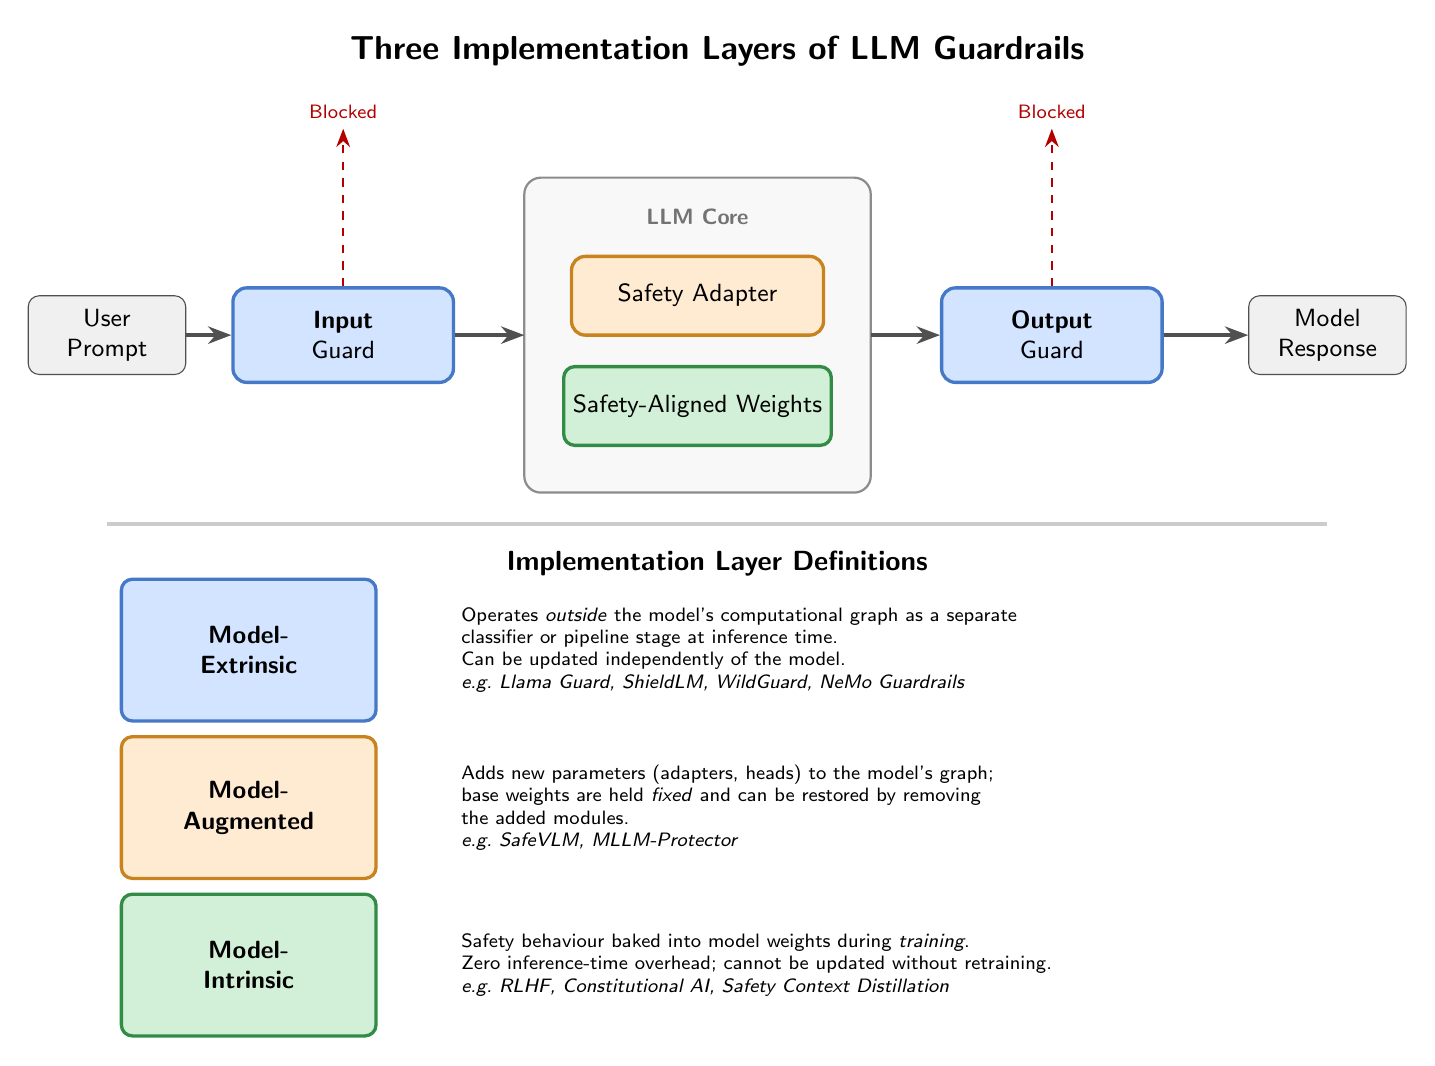
\begin{tikzpicture}[
  font=\sffamily,
  >=Stealth,
  %% ── node styles ────────────────────────────────────────────────────────────
  io/.style={
    rectangle, rounded corners=4pt,
    draw=clrArrow, fill=black!6,
    minimum width=2.0cm, minimum height=1.0cm,
    align=center, font=\small\sffamily
  },
  extrinsic/.style={
    rectangle, rounded corners=5pt,
    draw=clrExtrinsicBorder, fill=clrExtrinsic, very thick,
    minimum width=2.8cm, minimum height=1.2cm,
    align=center, font=\small\sffamily
  },
  augmented/.style={
    rectangle, rounded corners=5pt,
    draw=clrAugmentedBorder, fill=clrAugmented, very thick,
    minimum width=3.2cm, minimum height=1.0cm,
    align=center, font=\small\sffamily
  },
  intrinsicinner/.style={
    rectangle, rounded corners=4pt,
    draw=clrIntrinsicBorder, fill=clrIntrinsic, very thick,
    minimum width=3.2cm, minimum height=1.0cm,
    align=center, font=\small\sffamily
  },
  legbadge/.style={
    rectangle, rounded corners=4pt,
    very thick,
    minimum width=3.2cm, minimum height=1.0cm,
    align=center, font=\small\bfseries\sffamily
  },
  arrow/.style={->, very thick, clrArrow},
  blocked/.style={->, thick, red!70!black, dashed},
]

%%─────────────────────────────────────────────────────────────────────────────
%% LAYOUT CONSTANTS (all in cm)
%%   Pipeline y = 0
%%   x: prompt=0  extIn=3.0  llm=7.5  extOut=12.0  response=15.5
%%   LLM box: width=4.4cm, height=4.0cm → x: 5.3–9.7, y: −2.0–2.0
%%   Inside LLM:
%%     "LLM Core" label  y =  1.4   (top area, 0.6cm below LLM top)
%%     adapter           y =  0.5   height=1.0 → spans  0.0 to  1.0  (0.4cm below label)
%%     intrinsic         y = −0.9   height=1.0 → spans −1.4 to −0.4  (0.6cm gap from adapter bottom)
%%   Blocked arrows go to y = 2.6; title at y = 3.4
%%─────────────────────────────────────────────────────────────────────────────

%% ── Title ───────────────────────────────────────────────────────────────────
\node[font=\large\bfseries\sffamily] at (7.75, 3.6)
  {Three Implementation Layers of LLM Guardrails};

%% ── Pipeline nodes ──────────────────────────────────────────────────────────
\node[io]        (prompt)  at ( 0.0, 0) {User\\Prompt};
\node[extrinsic] (extIn)   at ( 3.0, 0) {\textbf{Input}\\Guard};
\node[extrinsic] (extOut)  at (12.0, 0) {\textbf{Output}\\Guard};
\node[io]        (response)at (15.5, 0) {Model\\Response};

%% ── LLM Core bounding box ───────────────────────────────────────────────────
%% Explicit rectangle so we control size precisely (width=4.4cm, height=4.0cm)
\draw[rounded corners=6pt, draw=black!45, fill=clrLLM, thick]
  (5.3, -2.0) rectangle (9.7, 2.0);
\node[font=\footnotesize\bfseries\sffamily, black!55] at (7.5, 1.5)
  {LLM Core};

%% ── Model-Augmented adapter (inside LLM, upper half) ────────────────────────
%% Center y=0.5; height=1.0cm → spans y=0.0 to y=1.0
%% Top clears LLM Core label (y=1.5 − font ≈ 0.35cm → label bottom ≈ 1.15, adapter top = 1.0) ✓
\node[augmented] (adapter)   at (7.5,  0.5) {Safety Adapter};

%% ── Model-Intrinsic weights (inside LLM, lower half) ────────────────────────
%% Center y=−0.9; height=1.0cm → spans y=−1.4 to y=−0.4
%% Gap between adapter bottom (y=0.0) and intrinsic top (y=−0.4) = 0.4cm ✓
%% Intrinsic bottom (y=−1.4) clears LLM box bottom (y=−2.0) by 0.6cm ✓
\node[intrinsicinner] (intrinsic) at (7.5, -0.9) {Safety-Aligned Weights};

%% ── Pipeline arrows ─────────────────────────────────────────────────────────
%% prompt → extIn: gap = extIn.left(1.6) − prompt.right(1.0) = 0.6cm ✓
\draw[arrow] (prompt.east)  -- (extIn.west);
%% extIn → LLM: gap = LLM.left(5.3) − extIn.right(4.4) = 0.9cm ✓
\draw[arrow] (extIn.east)   -- (5.3, 0);
%% LLM → extOut: gap = extOut.left(10.6) − LLM.right(9.7) = 0.9cm ✓
\draw[arrow] (9.7, 0)       -- (extOut.west);
%% extOut → response: gap = response.left(14.5) − extOut.right(13.4) = 1.1cm ✓
\draw[arrow] (extOut.east)  -- (response.west);

%% ── "Blocked" arrows ────────────────────────────────────────────────────────
%% extIn.north = y=0.6; arrow top = y=2.6; title bottom ≈ y=3.25 → gap 0.65cm ✓
\draw[blocked] (extIn.north)  -- ++(0, 2.0)
  node[above, font=\scriptsize\sffamily, red!70!black] {Blocked};
\draw[blocked] (extOut.north) -- ++(0, 2.0)
  node[above, font=\scriptsize\sffamily, red!70!black] {Blocked};

%%─────────────────────────────────────────────────────────────────────────────
%% LEGEND (below separator at y = −2.6)
%% Row centres: Extrinsic y=−3.6, Augmented y=−5.4, Intrinsic y=−7.2
%% Badge: x=1.8 (width=3.2cm → x: 0.2–3.4)
%% Text:  x=8.5 (text width=8.5cm → x: 4.25–12.75)  gap from badge right(3.4)=0.85cm ✓
%%─────────────────────────────────────────────────────────────────────────────

%% Separator line
\draw[black!20, very thick] (0.0, -2.4) -- (15.5, -2.4);

%% Legend header
\node[font=\normalsize\bfseries\sffamily] at (7.75, -2.9)
  {Implementation Layer Definitions};

%% ── Row 1: Model-Extrinsic ──────────────────────────────────────────────────
\node[legbadge,
  draw=clrExtrinsicBorder, fill=clrExtrinsic,
  minimum height=1.8cm, text width=3.0cm] at (1.8, -4.0)
  {\textbf{Model-\\Extrinsic}};
\node[text width=9.0cm, align=left, font=\scriptsize\sffamily] at (9.0, -4.0) {%
  Operates \emph{outside} the model's computational graph as a separate\\
  classifier or pipeline stage at inference time.\\
  Can be updated independently of the model.\\
  \textit{e.g.\ Llama Guard, ShieldLM, WildGuard, NeMo Guardrails}%
};

%% ── Row 2: Model-Augmented ──────────────────────────────────────────────────
\node[legbadge,
  draw=clrAugmentedBorder, fill=clrAugmented,
  minimum height=1.8cm, text width=3.0cm] at (1.8, -6.0)
  {\textbf{Model-\\Augmented}};
\node[text width=9.0cm, align=left, font=\scriptsize\sffamily] at (9.0, -6.0) {%
  Adds new parameters (adapters, heads) to the model's graph;\\
  base weights are held \emph{fixed} and can be restored by removing\\
  the added modules.\\
  \textit{e.g.\ SafeVLM, MLLM-Protector}%
};

%% ── Row 3: Model-Intrinsic ──────────────────────────────────────────────────
\node[legbadge,
  draw=clrIntrinsicBorder, fill=clrIntrinsic,
  minimum height=1.8cm, text width=3.0cm] at (1.8, -8.0)
  {\textbf{Model-\\Intrinsic}};
\node[text width=9.0cm, align=left, font=\scriptsize\sffamily] at (9.0, -8.0) {%
  Safety behaviour baked into model weights during \emph{training}.\\
  Zero inference-time overhead; cannot be updated without retraining.\\
  \textit{e.g.\ RLHF, Constitutional AI, Safety Context Distillation}%
};

\end{tikzpicture}
\end{document}
